\section{Requirements and System Model}\label{sec:requirements}
Big data is highly dependent on cloud-edge computing, which makes extensive use of multitenancy.
Multitenancy permits sharing one instance of infrastructures, platforms or applications by multiple tenants to optimize costs.
This leads to common scenarios where a service provider offers subscription-based analytics capabilities in the cloud,
or a single data lake is accessed by multiple customers.
Thus, it is a common situation to have a big data pipeline where data and services belong to various organizations,
posing a serious risk of potential privacy and security violation.
In the following of this section,
we present our system model (Section \ref{sec:systemmodel}),
the requirements driving our work (Section \ref{sec:accesscontrol_req}),
and our reference scenario (Section \ref{sec:reference}).
\AG{
  In our context a \user, aims to implement a data pipeline to facilitate analysis or transformation procedures on some data.
  Policies governing the data are established, which can originate from the \user, third-party entities, or regulatory frameworks.
  For instance, a policy may restrict the execution of processing operations to a specific geographic region.
  The \user is provided with a set of pipeline templates. Each template represents a blank pipeline with the necessary steps but without the specific services.
  To instantiate the template, the user is given the opportunity to choose, for each step of the pipeline, from a collection of candidate services that are functionally equivalent and comply with the specified policies.
  These services are subsequently ranked based on their ability to retain the maximum amount of data while maintaining an equivalent level of privacy.
  Underlying our investigation is the assumption that a greater quantity of preserved data corresponds to enhanced data quality.
}
\subsection{System Model}\label{sec:systemmodel}

\begin{itemize}
  \item User owns some data and wants to perform some analytics on it
  \item Choose a pipeline template and a wanted level of privacy
  \item The template has lambda, signed
  \item Policy is a set of rules
  \item Match the policy with the lambda
  \item Compares services that match the policy ranking them based on quality
  \item Choose the best service
  \item The composite service is executed
\end{itemize}

\AG{Our system model aims to achieve an optimal service composition to ensure privacy and data quality.
  Within this context, we contemplate an interconnected sequence of services, establishing a pipeline where individual nodes signify distinct services.
  Each stage within the pipeline undertakes the task of data transformation or processing, with the resulting output serving as the input for the subsequent service.
  This model encapsulates what we refer to as a template, visually presented in Figure \ref{fig:service_composition_template}.
  In order to instantiate the template, the selection of services to be executed at each step of the pipeline becomes imperative.
  At each step, there exists a collection of functionally equivalent services that differ in terms of annotation and data transformation.
  These services are annotated with a set of requirements that encompass crucial details, including the owner's information, as well as other pertinent metadata such as the region of execution, for example.
  The annotations play a pivotal role in the creation of policies that determine the eligibility of a service for deployment.
  By enforcing such policies, the set of candidate services for a given step is reduced.
  The remaining services undergo evaluation based on their potential impact on the data transformation process.
  Preference is given to the service that maximizes data quality while ensuring an equal level of data privacy.
  This evaluation process aids in identifying the most suitable service for a particular step in the pipeline.
  Upon the selection of the most appropriate service for each step, the instantiation of the pipeline is deemed complete.
  Consequently, the pipeline becomes ready for execution, with the assurance that the chosen services align with the specified requirements and optimize the desired outcomes.
}

% We formally model a Big Data analytics pipeline as follows.

% \begin{definition}[Big Data Analytics Pipeline] \label{def:pipeline}
%   A Big Data Analytics pipeline \G(\V,\E) is a direct acyclic graph having a root \vi{r}$\in$\V, a vertex \vi{i}$\in$\V$_I$$\subseteq$\V\ for each job \job{i} invocation, two additional vertices \vi{c},\vi{m}$\in$\V$_{\otimes}$$\subset$\V\ for each alternative ($\otimes$) structure modeling the alternative execution (\emph{choice}) of operations and the retrieval (\emph{merge}) of the results,
%     respectively, and two additional vertices \vi{f},\vi{j}$\in$\V$_{\oplus}$$\subset$\V\ for each parallel ($\oplus$) structure modeling the contemporary execution (\emph{fork}) of operations and the integration (\emph{join}) of their results, respectively.
% \end{definition}

% We note that each vertex \vi{i} model a job \job{i} provided by an organization \org{i}.
% We also note that an analytics pipeline can be deployed following a centralized or a decentralized approach as discussed in detail in Section \ref{sec:architecture}.

\begin{figure}[!t]
  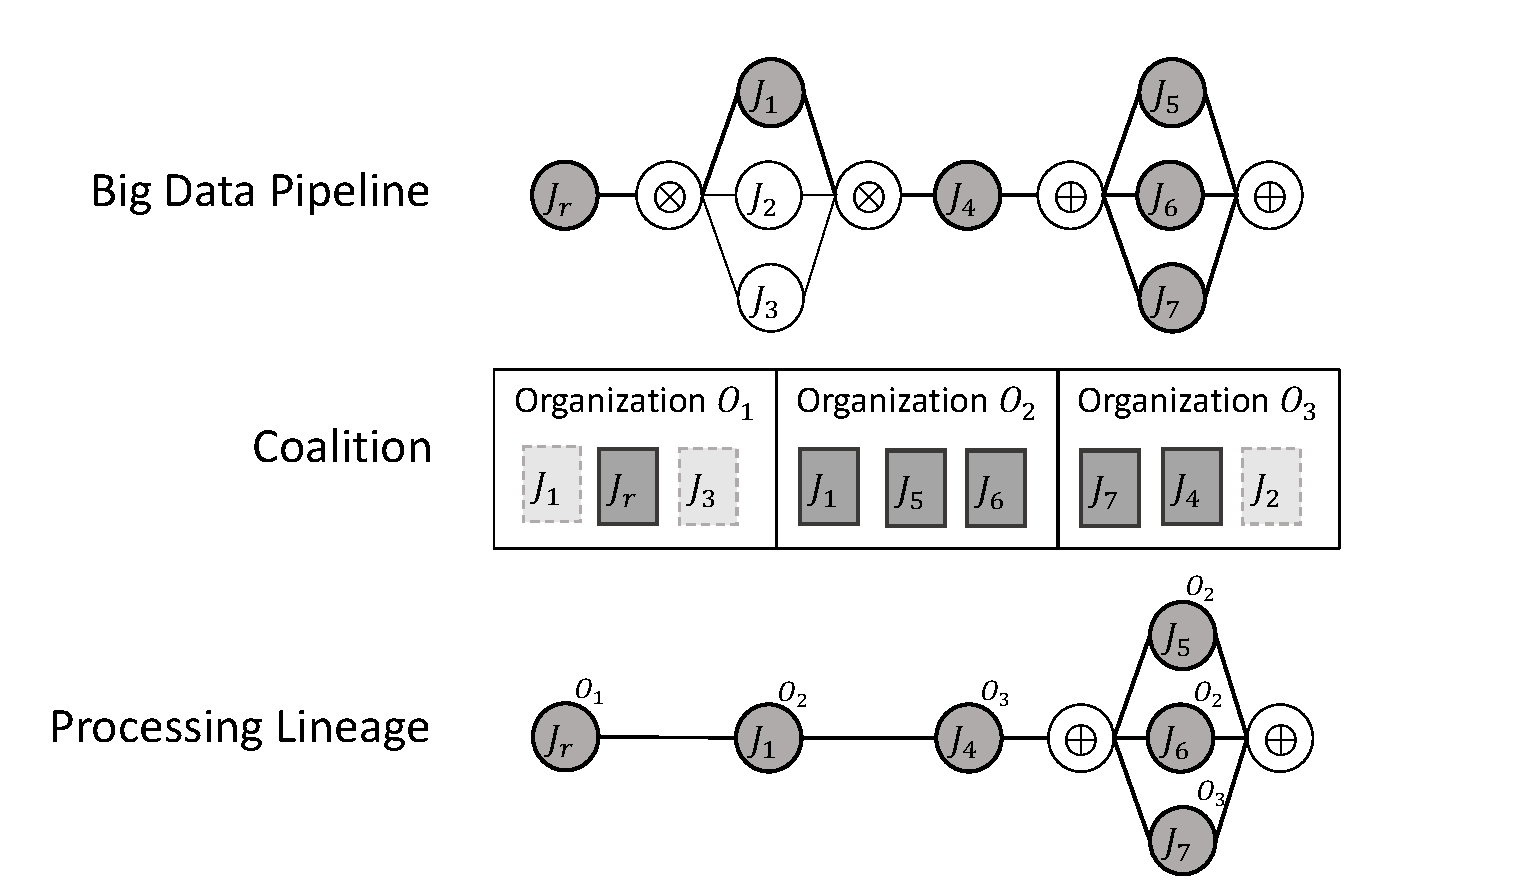
\includegraphics[width=0.98\columnwidth]{generaleFig1.pdf}
  \caption{Big Data Analytics pipeline graphs with a coalition of organization for a given processing lineage.}\label{fig:BDpipeline}
\end{figure}

Figure~\ref{fig:BDpipeline} shows an overview of our system model.

%Solid arrows present the typical batch or analytics model generation flows. Dashed arrows present typical streaming or prediction flows. \CH{togliere dalla figura la linea che separa le due procedure e le scritte ingestion procedure e analytics procedure?}
%The coalition creation is driven by missions including emergency and disaster management, humanitarian operations, or simply interdependent organizations.
%\CH{Qui ho introdotto solo il termine coalition, va spiegato anche il termine federation?}


\section{Policy}

\subsection{Annotations}
\subsection{Transformation}
\subsection{Policy}

\subsubsection{Policy Decision/Policy Matching}
\subsubsection{Policy Enforcement}
\subsubsection{Policy Evaluation}